\documentclass{article}

\usepackage{../../../preamble}

\title{3MD3020: Deep Learning Assignment}
\author{Raphael Reme}

\begin{document}
\maketitle


\section{Computer Vision Part}

% \paragraph{Question 1 -} Describe the steps needed to sample from such a model.
\subsection*{Question 1}

We have the following model:
\begin{equation*}
    \begin{aligned}
        z_n \sim  \mathcal{N}(0, I_D)                                                                                                                                        \\
        x_n^{(m)} | z_n \sim \mathcal{B}(f_\theta(z_n)_m) &  & \left(\Leftrightarrow p(x_n | z_n) = \prod_{m=1}^M\mathcal{B}\left(x_n^{(m)} ; f_\theta(z_n)_m\right) \right) \\
    \end{aligned}
\end{equation*}

We have $p(x_n) = \int_z p(x_n, z_n=z) dz = \int_z p(z_n=z)p(x_n | z_n = z) dz$. The ancestror sampling tells us here that sampling
$x_n$ is equivalent to sampling first $z_n$ and then sampling $x_n | z_n$. In our case it's handy as we know how to sample $z_n$ and $x_n | z_n$.

We can therefore first sample $z_n$ from the Gaussian distribution. Then we can sample each $x_n^{(m)} | z_n$ for $1 \le m \le M$ from a Bernouilli
distribution of mean $f_\theta(z_n))_m$. (Both easy to sample from with python).

\subsection*{Question 2}
% \paragraph{Question 2 -} Although Monte-Carlo Integration with samples from $p(z_n)$ can be used to approximate $\log p(x_n)$,
% it is not used for training VAE type of models, because it is inefficient. In a few sentences, describe why it is inefficient and
% how this efficiency scales with the dimensionality of $z$.

The Monte-Carlo Integration method approximate the expectation, but it converges at very a slow rate (in $\sqrt{L}$ from central limit theorem).
And more more over, we can rewrite the approximation:

\begin{equation*}
    \begin{aligned}
        p(x_n) & \approx \frac{1}{L}\sum_{l=1}^L p(x_n | z_l)                       \\
        p(x_n) & \approx \frac{1}{L}\sum_{l=1}^L p(x_n) \frac{p(z_l | x_n)}{p(z_l)} \\
    \end{aligned}
\end{equation*}

Thus we can see that we would like to avoid to sample too much $z$ such that $p(z | x_n) \approx 0$. And this becomes harder and harder when
$D$ increases. (The intuition is that $\{z \in \mathbb{R}^D, p(z) >\!\!> p(z | x_n)\}$ a bigger set for large dimension and that it's therefore
more frequent to sample $z$ such that $p(z | x_n) <\!\!< p(z)$.)

One can also have another intuition: The point of Monte Carlo is to sum enough samples so that the law of the sum converges to a dirac (centered
on the expectation, and of variance 0.). And the variance of this sum decreases in $\frac{1}{L}$. But it depends on the variance of the original law.
We can expect that the random variable $Y = p(x_n | Z)$ has a higher variance when $Z$ lives in a high dimensionnal space. And thus the sum of
sampled $Y$ has a bigger variance when $D$ increases (And we need a bigger $L$ to reach the same confidence in our approximation.)

\subsection*{Question 3}
Let's suppose $\sigma_p = \sigma_q = 1$.

Then:
\begin{equation*}
    \begin{aligned}
        D_{KL}(q || p) & = - \mathbb{E}_{x \sim q}\left[\log\frac{p(x)}{q(x)}\right]                                 \\
                       & = - \mathbb{E}_{x \sim q}\left[-\frac{1}{2} (x - \mu_p)^2 + \frac{1}{2}(x - \mu_q)^2\right] \\
                       & = - \mathbb{E}_{x \sim q}\left[(\mu_p - \mu_q)x - \frac{1}{2} (\mu_p^2 - \mu_q^2)\right]    \\
                       & = \frac{1}{2} (\mu_p^2 - \mu_q^2) -  (\mu_p - \mu_q) \mu_q                                  \\
    \end{aligned}
\end{equation*}
One can have a low value of $D_{KL}$ with $\mu_p = \mu_q = 0$: $D_{KL}(q || p) = 0$. And one can have a large value of $D_{KL}$ with $\mu_q = 0$
and a large $\mu_p$: $D_{KL}(q || p) = \frac{1}{2} \mu_p^2$.

\subsection*{Question 4}

We can show that the KL Divergence is a non negative number (using that $-\log(a) \ge 1 - a,\, \forall a > 0$).
Then it is obvious from $(16)$ that:

\begin{equation*}
    \log p(x_n) \ge \log p(x_n) - D_{KL}(q(Z | x_n) || p(Z | x_n)) = \mathbb{E}_{q(z_n|x_n)}\left[\log p(x_n | z_n)\right] - D_{KL}(q(Z | x_n) || p(Z))
\end{equation*}

As we don't know how to compute efficiently the log probability we can't optimize it directly. We rather maximizes a lower bound which
is tractable. (And the idea behind is that maximizing this lower bound will hopefully maximize our log probability.)


\subsection*{Question 5}

In this optimization process as we do not maximize $\log p(x_n)$ directly but $\log p(x_n) - D_{KL}(q(Z | x_n) || p(Z | x_n))$,
there are two possible things that can happen:
\begin{itemize}
    \item First, $\log p(x_n)$ increases, which is our goal. And in this situation our generative model is improving.
    \item Or $D_{KL}(q(Z | x_n) || p(Z | x_n))$ decreases. But it cannot decrease below 0 and therefore this possibility
          is limited. One can also notice that $q(z_n | x_n)$ was introduce to fit $p(z_n | x_n)$, in this situation, the approximation
          is getting better (as the KL divergence is reducing).
\end{itemize}

\subsection*{Question 6}
With $L_n^{\textbf{recon}} = - \mathbb{E}_{q_\phi(z|x_n)}\left[\log p_\theta(x_n | z) \right]$, one can observe that the minimization of this
loss is the maximization of the expectation. This is to say that given $x_n$ we try to find $\phi$ and $\theta$ such $q_\phi(z | x_n)$
is a law that will give high probability to $z$ such that $\log p_\theta(x_n | z)$ is also high. Meaning that we are learning
from $x_n$ to sample meaningful $z$ from which we can reconstruct $x_n$.

And for $L_n^{\textbf{reg}} = D_{KL}(q_\phi(Z | x_n) || p(Z))$ we enforce the law $q_\phi( Z | x_n)$ to be close
enough to $p(Z)$ which is a simple Gaussian: $\mathcal{N}(0, I_D)$. It acts therefore as a regularizer !

\subsection*{Question 7}

First, in order to approximate $L_n^{\textbf{recon}} = - \mathbb{E}_{q_\phi(z|x_n)}\left[\log p_\theta(x_n | z) \right]$ we will do a
Monte Carlo approximation with only one sample: We will sample $z_n$ and:

\begin{equation*}
    \begin{aligned}
        L_n^{\textbf{recon}} & \approx - \log p_\theta(x_n | z_n)                                                                               \\
                             & \approx - \log \prod_{m=1}^M\mathcal{B}\left(x_n^{(m)} ; f_\theta(z_n)_m\right)                                  \\
                             & \approx - \sum_{m=1}^M \left( x_n^{(m)} \log f_\theta(z_n)_m + (1 - x_n^{(m)}) \log(1 - f_\theta(z_n)_m) \right)
    \end{aligned}
\end{equation*}

We can notice that this is the binary cross entropy between $x_n$ and the reconstructed $f_\theta(z_n)$!

Then in order to compute $L_n^{\textbf{reg}} = D_{KL}(q_\phi(Z | x_n) || p(Z))$. We will use that $p(z_n) = \mathcal{N}(z_n; 0, I_D)$
and $q_\phi(z_n | x_n) = \mathcal{N}(z_n; \mu_\phi(x_n), \text{Diag}(\Sigma_\phi(x_n)))$ and equation $(9)$. I will first compute the left
term. (Note that our definition of $q_\phi$ with a diagonal matrix as a covariance matrix will help us)

\begin{equation*}
    \begin{aligned}
        - \int_z q_\phi(z | x_n) \log p(z) dz & = - \int_z q_\phi(z | x_n) \log\left( \frac{1}{(2\pi)^{D/2}} \exp\left(-\frac{1}{2}z^Tz\right)\right)dz           \\
                                              & = \frac{D}{2}\log(2\pi) + \frac{1}{2} \int_z q_\phi(z | x_n) z^Tz dz                                              \\
                                              & = \frac{D}{2}\log(2\pi) + \frac{1}{2} \mathbb{E}_{q_\phi(z | x_n)}\left[\sum_i z_{i}^2\right]                     \\
                                              & = \frac{D}{2}\log(2\pi) + \frac{1}{2} \sum_i \Sigma_\phi(x_n)_i + \mu_\phi(x_n)_i^2                               \\
                                              & = \frac{D}{2}\log(2\pi) + \frac{1}{2} \mathds{1}_D^T\Sigma_\phi(x_n) + \frac{1}{2}  \mu_\phi(x_n)^T \mu_\phi(x_n) \\
    \end{aligned}
\end{equation*}

And we can do the same calculation for the second term, we can notice that $|\text{Diag}(\Sigma_\phi(x_n))| = \prod_i \Sigma_\phi(x_n)_i$
and that $\text{Diag}(\Sigma_\phi(x_n))^{-1} = \text{Diag}(\frac{1}{\Sigma_\phi(x_n)})$. This gives us:

\begin{equation*}
    \begin{aligned}
        \int_z q_\phi(z | x_n) \log q_\phi(z | x_n) dz & = -\frac{D}{2}\log(2\pi) - \frac{1}{2}\log|\text{Diag}(\Sigma_\phi(x_n))| - \frac{1}{2} \int_z q_\phi(z | x_n) (z - \mu_\phi(x_n))^T \text{Diag}(\Sigma_\phi(x_n))^{-1} (z - \mu_\phi(x_n))dz \\
                                                       & = -\frac{D}{2}\log(2\pi) - \frac{1}{2} \mathds{1}_D^T\log \Sigma_\phi(x_n) - \frac{1}{2} \int_z q_\phi(z | x_n) \sum_i \frac{1}{\Sigma_\phi(x_n)_i} (z_i - \mu_\phi(x_n)_i)^2 dz              \\
                                                       & = -\frac{D}{2}\log(2\pi) - \frac{1}{2} \mathds{1}_D^T\log \Sigma_\phi(x_n) - \frac{1}{2} \sum_i \frac{1}{\Sigma_\phi(x_n)_i} \mathbb{E}_{q_\phi(z | x_n)}[(z_i - \mu_\phi(x_n)_i)^2]          \\
                                                       & = -\frac{D}{2}\log(2\pi) - \frac{1}{2} \mathds{1}_D^T\log \Sigma_\phi(x_n) - \frac{1}{2} \sum_i \frac{1}{\Sigma_\phi(x_n)_i} \Sigma_\phi(x_n)_i                                               \\
                                                       & = -\frac{D}{2}\log(2\pi) - \frac{1}{2} \mathds{1}_D^T\log \Sigma_\phi(x_n) - \frac{1}{2} D                                                                                                    \\
    \end{aligned}
\end{equation*}
We have therefore:

\begin{equation*}
    \begin{aligned}
        L_n^{\textbf{reg}} & = D_{KL}(q_\phi(Z | x_n) || p(Z))                                                                                                     \\
                           & = - \int_z q_\phi(z | x_n) \log p(z) dz + \int_z q_\phi(z | x_n) \log q_\phi(z | x_n) dz                                              \\
                           & =  \frac{1}{2}\left(\mathds{1}_D^T\Sigma_\phi(x_n) + \mu_\phi(x_n)^T \mu_\phi(x_n) - \mathds{1}_D^T\log \Sigma_\phi(x_n) - D  \right) \\
    \end{aligned}
\end{equation*}

Finally all we have to do is to sample $z_n$ from the current $q_\phi(z|x_n)$ for each $n$ and then we can compute the losses for these data.

\subsection*{Question 8}

One can see that $L_n^{\textbf{recon}}$ depends on $\phi$ and $\theta$ and that we want to compute its gradient w.r.t two both of the
parameters.
But the list of operations that links $\phi$ to $L_n^{\textbf{recon}}$ contains a sampling operation: We sample from $q_\phi(z | x_n)$ and
this is not a differentiable operation and thus the gradient can't be computed without a trick.

The reparametrization trick consists in sampling $\epsilon \sim \mathcal{N}(0, I_D)$ and then compute
$z = \mu_\phi(x_n) + \text{Diag}(\Sigma_\phi(x_n)^{\frac{1}{2}}) \times \epsilon$. Then one can see that $z \sim \mathcal{N}(\mu_\phi(x_n), \Sigma_\phi(x_n))$.
We have thus generate from $\epsilon$ a sample following the law of $q_\phi(z | x_n)$. But this times the dependencies in $\phi$ are differentiable
as we only use sum and product to compute this sample (from $\epsilon$). We will be able to compute the gradient of $L_n^{\textbf{recon}}$
w.r.t. $\phi$

(And all the other gradients are computable)

\subsection*{Question 9}
I will use the very basic architecture (We'll see that it is enough) for the encoder and decoder. They both will be Sequential networks
with two layers and a ReLU activation to separate them. The input dimension is $28 \times 28 = 784$ and the latent dimension is chosen
to be $20$. I made the choice of an intermiate hidden dimension of $350$.

Therefore the encoder is composed of one Linear Layer of shape $(784, 350)$ and another of shape $(350, 2 \times 20)$
(As it predicts $\mu$ and $\Sigma$). And the decoder is composed of one layer $(20, 350)$ and another $(350, 784)$.
I did not put a Sigmoid at the end of the decoder and I rather uses directly a Binary Cross Entropy with Logits (implemented by pytorch).

I will use Adam which is often more stable SGD and a learning rate of 0.001 has proven itself to be the best. I will
consider batch of the dataset of size 64, for each of them I will compute the loss as explained in $Q7$ and use automatic
differentiation to do the back propagation. (I averaged the loss on the batch in order to keep the same order of loss for different batch
sizes)

\subsection*{Question 10}
The results can be reproduce with:

\begin{lstlisting}{bash}
    $ python main_vae.py 0 10 80
\end{lstlisting}

We are able to generate new images from a $\mathcal{N}(0, I_D)$ (\ref{fig:MLP}) (I tried also to visualize reconstructed image
from a given existing image. They are of course much better that those generated here without initial image to encode.)

\begin{figure}[ht]
    \centering
    \begin{subfigure}[b]{0.3\linewidth}
        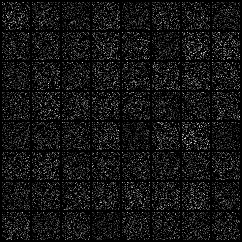
\includegraphics[width=\linewidth]{mlp_0.png}
    \end{subfigure}
    \begin{subfigure}[b]{0.3\linewidth}
        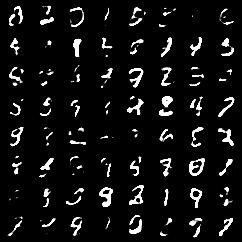
\includegraphics[width=\linewidth]{mlp_10.png}
    \end{subfigure}
    \begin{subfigure}[b]{0.3\linewidth}
        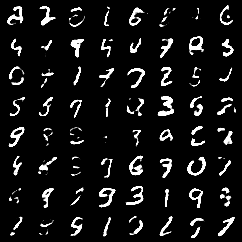
\includegraphics[width=\linewidth]{mlp_80.png}
    \end{subfigure}
    \caption{Generated images by the MLP Vae at epochs 0, 10, 80. The same $z \sim \mathcal{N}(0, I_D)$ is used for the 3 images}
    \label{fig:MLP}
\end{figure}

One can observe that initially we are juste generating noise. And after only 10 epochs the model is able to generate images that are similar
to digits. It has learned that the background is black and some of the white drawings are looking very similar to digits. After 80 epochs, the
model seems a little bit better, digits have improved even though there are still some of them that seems to be either a mixed of digits,
or just a shade of a digit.

Indeed as the model is continuous it sometimes output an image which is similar to several digits. And it also sometimes outputs a mostly
black (empty) image, which is understandabe as black is the main color of the dataset images, it will suffer less loss predicting empty images
(or what I called shade images, where we have just some parts not very visible of digits.)

\subsection*{Question 11}

I choose to use an architecture slightly different from UNet: First we can't use the idea of skip connections of the UNet architecture as it
would create skip connections between the images and the decoder (the network will cheat and use the initial image to reconstruct it and not
the sampled latent variable. And it won't be able to reconstruct an image from the latent space only.)

I choose nonetheless to keep the idea of reducing the dimension with convolution and maxpooling for the decoder and uses up-convolution in
the decoder to get back to the 28x28 shape. I found out that batch normalization helped a lot the network (I was unable to train
successfully my networks without it.)

My final convolution encoder is therefore a succession of 2D convolutions with batch normalization and ReLU followed by a max pooling. Rather
than padding the input image in a 32x32 shape (much easier to divide the shape by 2) I adapted the padding in order to decreases the shape
up to 1x1 (with 40 features). I have therefore kept a latent space of dimension (20, 1, 1).

The decoder performs 4x4 up-convolution from this latent space with batch normalization and ReLU until it reaches the 28x28 input dimension.
(I also adapted the padding as needed).

I trained this architecture with Adam and a learning rate of 0.001 and it has yields better results than with the MLP encoder/decoder vae.

\begin{lstlisting}{bash}
    $ python main_vae.py -a conv 0 10 80
\end{lstlisting}

\begin{figure}[ht]
    \centering
    \begin{subfigure}[b]{0.3\linewidth}
        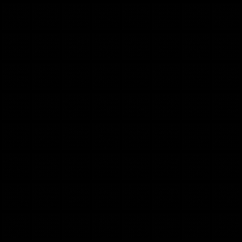
\includegraphics[width=\linewidth]{conv_0.png}
    \end{subfigure}
    \begin{subfigure}[b]{0.3\linewidth}
        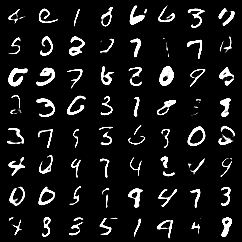
\includegraphics[width=\linewidth]{conv_10.png}
    \end{subfigure}
    \begin{subfigure}[b]{0.3\linewidth}
        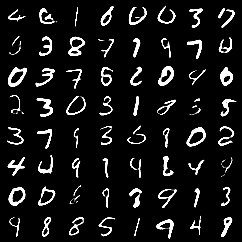
\includegraphics[width=\linewidth]{conv_80.png}
    \end{subfigure}
    \caption{Generated images by the Conv Vae at epochs 0, 10, 80.}
    \label{fig:conv}
\end{figure}


We can see that the digits generated are really good. There are still some digits that are ambiguous but much less than with the MLP encoder.


\subsection*{Question 12}
It seems that the attention matrixes are not really well generated. I will just comment some of the key idea on some attention matrixes
from \cite{attention}.

\begin{figure}[h!]
    \centering
    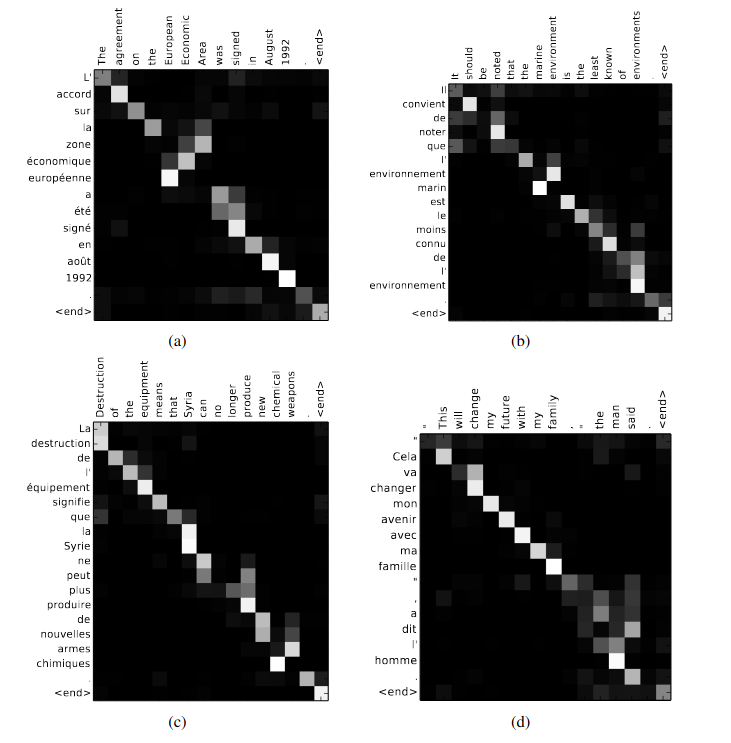
\includegraphics[width=0.6\linewidth]{attention.png}
    \caption{Attention matrixes \cite{attention}}
    \label{fig:attention}
\end{figure}

On these attention matrixes one can see immediately that the words used by the network through attention in order to predict the next
are the relevant ones.

They are often on the diagonal but not always. We can take for instance the first example:
"The agreement on the European Economic Area was ..." $\rightarrow$ "L'accord sur la zone économoique européenne a été ...".

We have an example of traduction where the attention is not on the diagonal because of some words inversion: "zone" has been mainly
translated thanks to the embedding of "Area" and "Economic" which are placed before European in the English sentence.
One can also notice the word "la" where the translation comes from "the" but the gender is extracted from "zone" and the attention is
on these two words.


\subsection*{Question 13}

In these settings, the encoder has to encode the input sentence and the decoder has to use this embeddings to produce the output sentence.

Without attention, the encoder outputs a single vector that represents the whole sentence which is used by the decoder (here as initial hidden
state). The decoder has to extract from this vector the first word and the second and the others, which is a hard task. One could also think
to give to the decoder at time $t$ the $t^\text{th}$ encoded word. But words from two different languages are not aligned on the same
position and thus it won't work well. (This attention mechanism will allow the decoder to solve this alignment problem)

Here attention allows the network to combine the current hidden state and last predicted word with all the outputs of the encoder and
extract what matters at this particular moment. The encoder has no longer to produce a single vector responsible for the whole input sentence.
And the decoder is able to select what matters for him at each time step and thus to select which are the encoded words to use for its
next output.

\subsection*{Question 14}
In the decoder network, we use the previous output as next input. In this kind of settings, a mistake done by the network will probably leads
to another mistake for the next word prediction. And in the training phase this will reduce the training efficiency.

The idea behind teacher forcing is to use as next input the real previous token rather than the predicted previous token. This improves
training as when we are wrong at a point in the sequence the input used to continue is still the good one, allowing us to keep trying to fit the
end of the sequence (which would have been much harder from a wrong input).

But the drawback is that the network learned can rely to much on the teacher and does not learn to perform the task by itself.
Therefore in this tutorial they only randomly use teacher forcing half of the time.

\subsection*{Question 15}
Using the same calculations we have:

\begin{equation*}
    \frac{\partial e}{\partial x_\ell} = \frac{\partial e}{\partial x_L} \prod_{i=\ell}^{L-1} \frac{\partial x_{i+1}}{\partial x_i}
\end{equation*}

Then from equation $(21)$ we can write:
\begin{equation}
    \tag{21'}
    \begin{aligned}
        \frac{\partial x_{\ell + 1}}{\partial x_\ell} & = \frac{\partial (x_\ell + A(x_\ell))}{x_\ell}\frac{\partial \text{LayerNorm}(x_\ell + A(x_\ell))}{\partial (x_\ell + A(x_\ell))}                         \\
                                                      & = \left(\mathbf{1} + \frac{\partial A(x_\ell)}{\partial x_\ell}\right)\frac{\partial \text{LayerNorm}(x_\ell + A(x_\ell))}{\partial (x_\ell + A(x_\ell))}
    \end{aligned}
\end{equation}

Whereas from equation $(22)$ we do not have the same result:
\begin{equation*}
    \tag{22'}
    \begin{aligned}
        \frac{\partial x_{\ell + 1}}{\partial x_\ell} & = \mathbf{1} + \frac{\partial A(\text{LayerNorm}(x_\ell))}{x_\ell}                                                                                      \\
                                                      & = \mathbf{1} + \frac{\partial \text{LayerNorm}(x_\ell)}{\partial x_\ell} \frac{\partial \text{A(LayerNorm}(x_\ell))}{\partial \text{LayerNorm}(x_\ell)}
    \end{aligned}
\end{equation*}


In the $(22')$ case we have a real skip connection and the $1$ constant is in all the terms of the product in $\frac{\partial e}{\partial x_\ell}$.

\subsection*{Question 16}
In a very deep architecture that relies on equation $(21)$ rather the $(22)$ we could end up in a situation of vanishing gradient as
the skip connections are not entirely skipped: If the LayerNorm operation induces at each step a reduction of the gradient, the first
layers of a deep architecture will face a vanished gradient in the back propagation.

Let's for instance suppose that we have
\begin{equation*}
    \left|\frac{\partial \text{LayerNorm}(x_i + A(x_i))}{\partial (x_i + A(x_i))} \right| \le \lambda < 1
\end{equation*}
We would then have a vanishing gradient problem:
\begin{equation*}
    \left|\frac{\partial e}{\partial x_\ell}\right| < \left| \frac{\partial e}{\partial x_L}\prod_{i=\ell}^{L-1} \left(1 + \frac{\partial A(x_\ell)}{\partial x_\ell}\right )\right| \lambda^{L - \ell - 1}
\end{equation*}

On the other hand with equation $(22)$ we have a true skip connection, and thus vanishing gradient problem cannot occur by simply stacking these
layers.

\subsection*{Question 17}

{\small
    \bibliographystyle{plain}
    \bibliography{biblio}
}

\end{document}
